% \documentclass [11pt, a4paper]{beamer}
% \usetheme {CambridgeUS}
% \usepackage [utf8]{inputenc}
% \usepackage [portuguese]{babel}
% \usepackage{verbatim}
% \usepackage{graphicx}
% \usepackage{url}
% \usepackage{multicol}

% %%% These packages for listing LaTeX code inside beamer
% \usepackage{listings}
% \usepackage{color}

% \definecolor{lightgrey}{rgb}{0.9,0.9,0.9}
% \definecolor{darkgreen}{rgb}{0,0.6,0}

% % Informations about the presentation
% \title {Introdução ao \LaTeX{}}
% \subtitle{Uma Abordagem Prática}
% \author[Danilo, Luiz, Pablo]{
%     Danilo S. Oliveira\\
%     Luiz S. Oliveira\\
%     Pablo A. A. Urbizagastegui
% }
% \institute[]{Universidade de Brasília}
% \date {\today}

% % To eliminate navigation buttons
% \setbeamertemplate{navigation symbols}{}

% % Includes logo on the layout of the document
% \logo{
%   
\includegraphics[scale=0.18]{figuras/cdt} \hspace{4.2cm}
%   
\includegraphics[scale=0.2]{figuras/lab}   \hspace{4.0cm}
%   
\includegraphics[scale=0.05]{figuras/unb}
% }

% % Delete this, if you do not want the table of contents to pop up at
% % the beginning of each subsection or section:
% \AtBeginSection[]{
%     \begin{frame}<beamer>{Conteúdo}
%         \tableofcontents[currentsection]
%     \end{frame}
% }

% \begin {document}

% \frame{\titlepage}

\begin {frame}{Conteúdo}
\small
    \begin{multicols}{3}
        \tableofcontents
    \end{multicols}
\end {frame}

\section {\TeX{} /\LaTeX{}}
\subsection {Histórico}
\begin{frame}
\begin{figure}[htbp]
    \centering
        
\includegraphics[width=0.5\textwidth]{figuras/tipografia.jpeg}
    \caption{Tipografia}
    \label{fig:tipografia}
\end{figure}
\end{frame}

\subsection {Apresentação}
\begin{frame}{\TeX{}}
    \begin{itemize}
        \item Sistema tipográfico criado por Donald Knuth na década de 80.
        \item Voltado para a tipografia de textos e fórmulas matemáticas.
        \item É extremamente estável e apresenta pouquíssimos \textit{bugs}.
        \item Não fornece muitas abstrações úteis para a confecção de um texto.
    \end{itemize}
\begin{figure}[htbp]
    \centering
    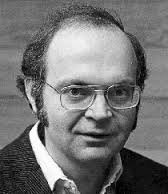
\includegraphics[width=0.15\textwidth]{figuras/donald.jpeg}
    \caption{Donald Knuth}
    \label{fig:tipografia}
\end{figure}
\end{frame}

\begin{frame}{\LaTeX{}}
    \begin{itemize}
        \item Criado por Leslie Lamport, é um conjunto de macros para o \TeX{}, facilitando a utilização de seu sistema tipográfico.
        \item Criado com a ideia de que o autor não deveria se preocupar com a formatação do texto, mas apenas em sua estrutura.
    \end{itemize}
    \begin{figure}[htbp]
    \centering
    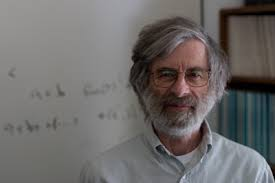
\includegraphics[width=0.25\textwidth]{figuras/leslie.jpeg}
    \caption{Leslie Lamport}
    \label{fig:leslie}
\end{figure}
\end{frame}

\begin{frame}
\begin{figure}[htbp]
    \centering
        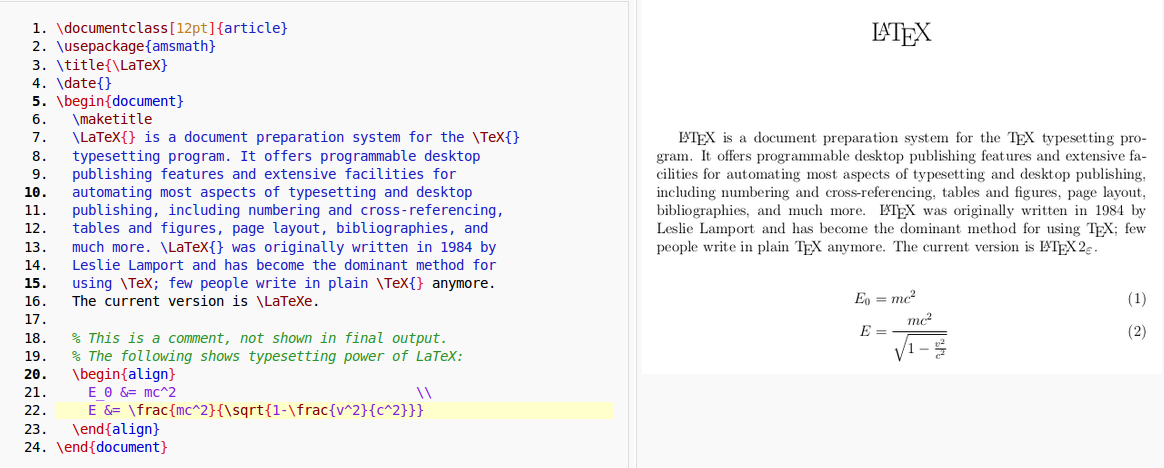
\includegraphics[width=1\textwidth]{figuras/output.png}
    \caption{http://en.wikipedia.org/wiki/LaTeX}
    \label{fig:output}
\end{figure}
\end{frame}

\section{Vantagens e Desvantagens}
\subsection{Vantagens}
\begin{frame}{Vantagens}
\begin{columns}[T]
    \begin{column}[T]{5cm}
        \begin{itemize}
            \item Software Livre;
            \item Alta qualidade tipográfica;
            \item Formatações automática dos textos;
            \item Extremamente customizável;
            \item Facilita a escrita de documentos com expressões matemáticas.
        \end{itemize}
    \end{column}

    \begin{column}[T]{5cm}
        \centering
        
\includegraphics[height=4cm]{figuras/hq.png}
        %http://www.somethingofthatilk.com/index.php?id=135
    \end{column}
\end{columns}
\end{frame}

\subsection{Desvantagens}

\begin{frame}{Desvantagens}
\begin{itemize}
    \item Embora a utilização de estilos prontos de documento seja fácil, a criação de novos modelos leva muito tempo;
    \item É muito difícil escrever documentos fora de um padrão ou template;
    \item A aprendizagem é mais difícil que em editores de texto comuns.
\end{itemize}
\end{frame}

\section{Links Importantes}
\subsection{}
\begin{frame}{Fontes Importantes}
  \begin{thebibliography}{10}
  \beamertemplatearticlebibitems
  \bibitem{wiki}
    http://en.wikibooks.org/wiki/LaTeX
    \newblock \href{http://en.wikibooks.org/wiki/LaTeX}{\beamergotobutton{Link}}
    \bibitem{ctan}
    http://ctan.org/
    \newblock \href{http://ctan.org/}{\beamergotobutton{Link}}
    \bibitem{stack}
    http://tex.stackexchange.com/
    \newblock \href{http://tex.stackexchange.com/}{\beamergotobutton{Link}}
  \end{thebibliography}
\end{frame}

% \end{document}